\documentclass[a4paper, 12pt]{article}
\usepackage[utf8x]{inputenc}
\usepackage{cmap}
\usepackage[english, russian]{babel}
\usepackage{indentfirst}
\usepackage[left=20mm, top=20mm, right=20mm, bottom=20mm]{geometry}
\usepackage{tikz}
\usepackage{float}
\usepackage{amsmath, amsfonts, amssymb}
\usepackage{graphicx}
\usepackage{fancybox, fancyhdr}
\usepackage{hyperref}
\usepackage{listings}
\usepackage{caption}
\usepackage{subcaption}
\usepackage{xcolor}
\pagestyle{fancy}
\fancyhf{}
\fancyhead[L]{Лабораторная работа №4}
\fancyhead[R]{Частотные методы}
\fancyfoot[C]{\thepage}
\graphicspath{{images/}}
\usetikzlibrary{patterns}
\definecolor{LightGray}{gray}{0.95}
\lstdefinestyle{pycode}{
    language=Python,
    basicstyle=\footnotesize\ttfamily,
    numbers=left,
    numberstyle=\tiny\color{gray},
    stepnumber=1,
    numbersep=5pt,
    backgroundcolor=\color{LightGray},
    showspaces=false,
    showstringspaces=false,
    showtabs=false,
    tabsize=4,
    captionpos=b,
    breaklines=true,
    breakatwhitespace=false,
    frame=none,
    rulecolor=\color{black},
    linewidth=\linewidth,
    keywordstyle=\color{red}\bfseries,
    commentstyle=\color{green!40!black},
    stringstyle=\color{blue},
    escapeinside={\%*}{*)},
    xleftmargin=0pt,
    framexleftmargin=0pt,
    framexrightmargin=0pt
}
\lstset{style=pycode}
\hypersetup{
    colorlinks=true,
    linkcolor=blue,
    filecolor=magenta,
    urlcolor=cyan,
    pdftitle={contents setup},
    pdfpagemode=FullScreen,
}
\setlength{\parskip}{1.5mm}
\setlength{\headheight}{15pt}
\setlength{\footskip}{15pt}
\allowdisplaybreaks
\DeclareMathOperator{\sinc}{sinc}
\newcommand{\frc}[2]{\raisebox{2pt}{$#1$}\big/\raisebox{-3pt}{$#2$}}

\begin{document}
    \begin{titlepage}

        \begin{center}
        
\includegraphics[width=0.3\textwidth]{itmo.png} % requires itmo.png in /images folder
        \vfill

        Федеральное государственное автономное образовательное учреждение высшего образования
        «Национальный Исследовательский Университет ИТМО»\\

        \vfill
        {\large\bf ЛАБОРАТОРНАЯ РАБОТА №4}\\
        {\large\bf ПРЕДМЕТ «ЧАСТОТНЫЕ МЕТОДЫ»}\\
        {\large\bf ТЕМА «ЛИНЕЙНАЯ ФИЛЬТРАЦИЯ»}
        \vfill

        \begin{flushright}
            \begin{minipage}{.45\textwidth}
            {
                \hbox{Лектор: Перегудин А. А.}
                \hbox{Практик: Пашенко А. В.}
                \hbox{Студент: Румянцев А. А.}
                \hbox{Поток: ЧАСТ.МЕТ. 1.3}
                \hbox{}
                \hbox{Факультет: СУиР}
                \hbox{Группа: R3241}
            }
            \end{minipage}
        \end{flushright}

        \vfill

        Санкт-Петербург\\
        2024
        \end{center}
    \end{titlepage}

    \tableofcontents

    \newpage
    \section{Задание 1. Спектральное дифференцирование.}
    Зададим в python список $t$ от $-100$ до $100$ включительно с шагом $dt$ и рассмотрим зашумленный сигнал вида $$y=\sin{(t)}+a\cdot(\text{rand}(\text{len}(t))-0.5).$$
    Построим соответствующий график при переменных $a=0.2,\,dt=0.25$. На всех графиках в названии указываются значения используемых параметров для удобства рассматривания
    различных результатов и последующего сравнения.
    \begin{figure}[H]
        \centering
        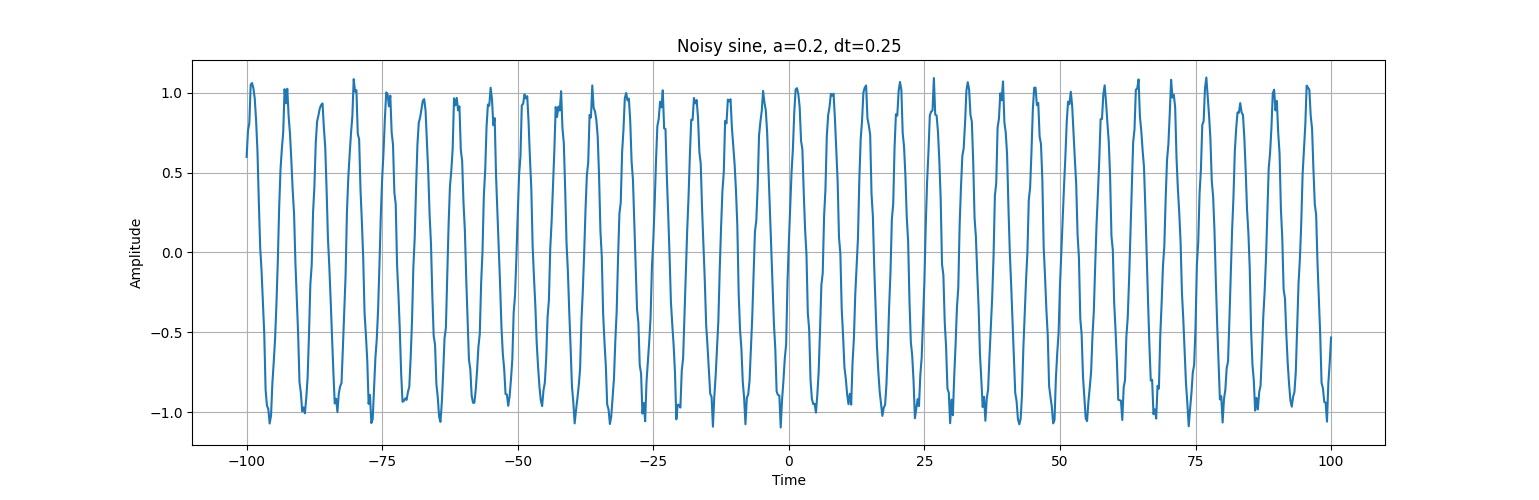
\includegraphics[scale=0.4]{1_noisy_sine.png}
        \captionsetup{skip=0pt}
        \caption{График зашумленного сигнала.}
        \label{fig:1ns}
    \end{figure}
    Найдем численную производную от данного сигнала, используя формулу поэлементного дифференцирования $$\dfrac{y(k+1)-y(k)}{dt},$$ после чего построим график.
    \begin{figure}[H]
        \centering
        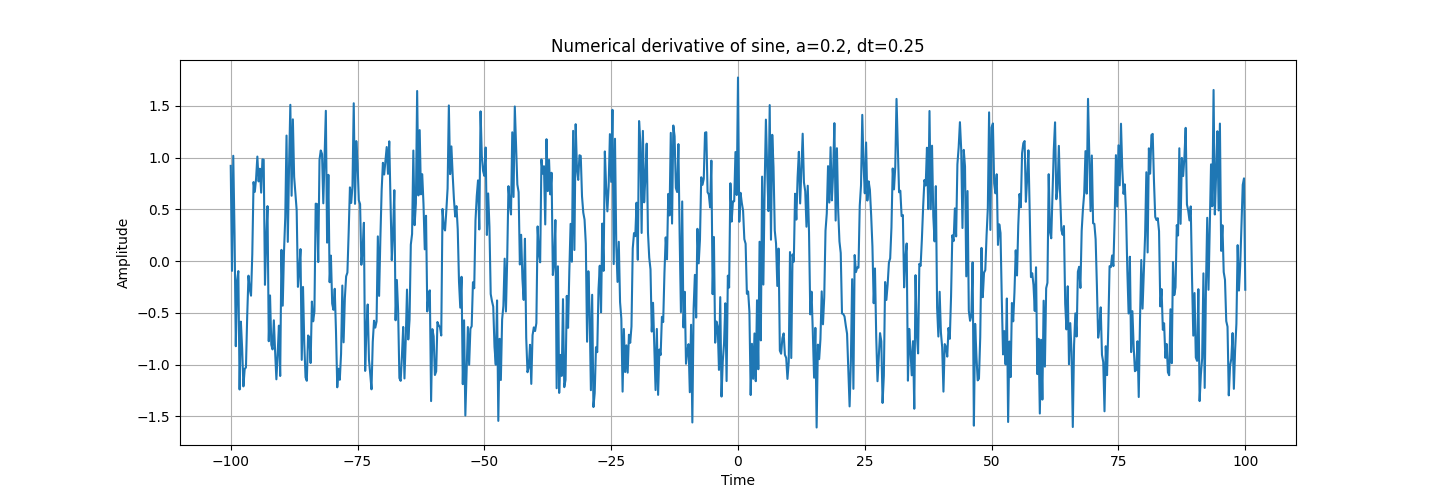
\includegraphics[scale=0.4]{1_numdiff_sine.png}
        \captionsetup{skip=0pt}
        \caption{Численная производная зашумленного сигнала.}
        \label{fig:1nds}
    \end{figure}
    Найдем спектральную производную от зашумленного сигнала. Для прямого и обратного преобразования Фурье будем использовать численное интегрирование (trapz). Чтобы
    превратить Фурье-образ сигнала в Фурье-образ производной, необходимо домножить результат преобразования Фурье на $2\pi i \nu$, где $\nu$ -- частота (Гц),
    таким образом получим формулу $$\mathcal{F}\left\{\frac{d}{dt}f\right\}=2\pi i \nu \mathcal{F}\left\{f\right\}.$$ Теперь остается только выполнить обратное преобразование Фурье, чтобы получить
    спектральную производную сигнала. Далее приведен соответствующий график. Так как у спектральной производной есть вещественная и мнимая части, рассмотрим их отдельно.
    \begin{figure}[H]
        \centering
        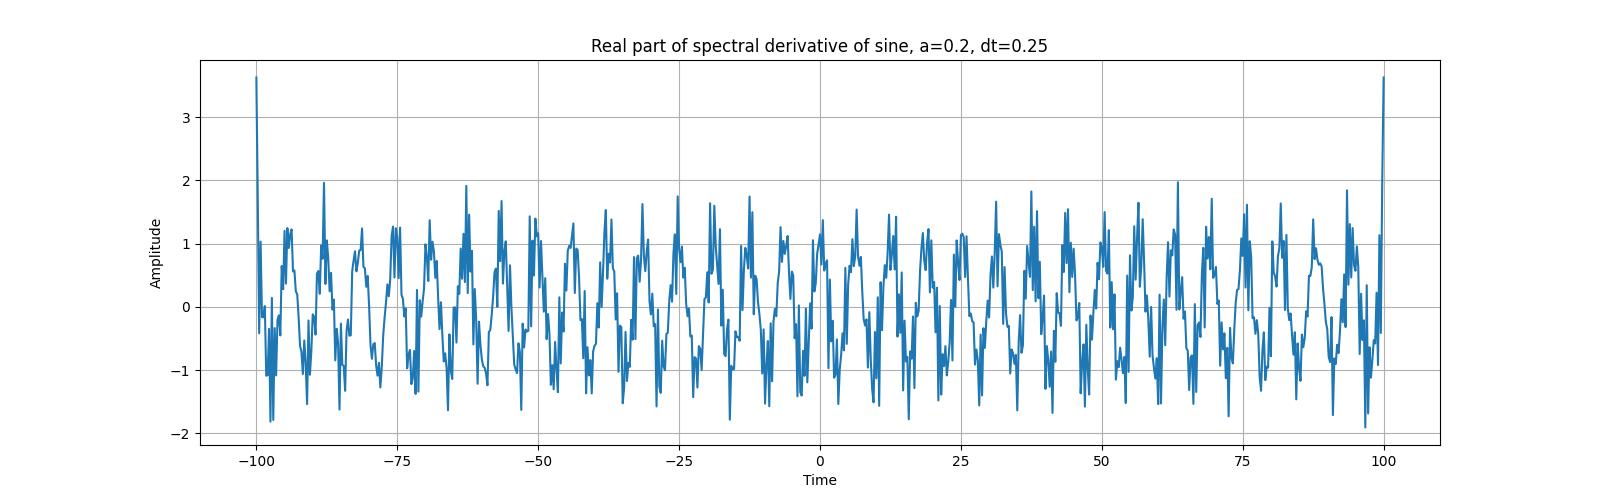
\includegraphics[scale=0.4]{1_re_specdiff_sine.png}
        \captionsetup{skip=0pt}
        \caption{Вещественная часть спектральной производной зашумленного сигнала.}
        \label{fig:1respd}
    \end{figure}
    \begin{figure}[H]
        \centering
        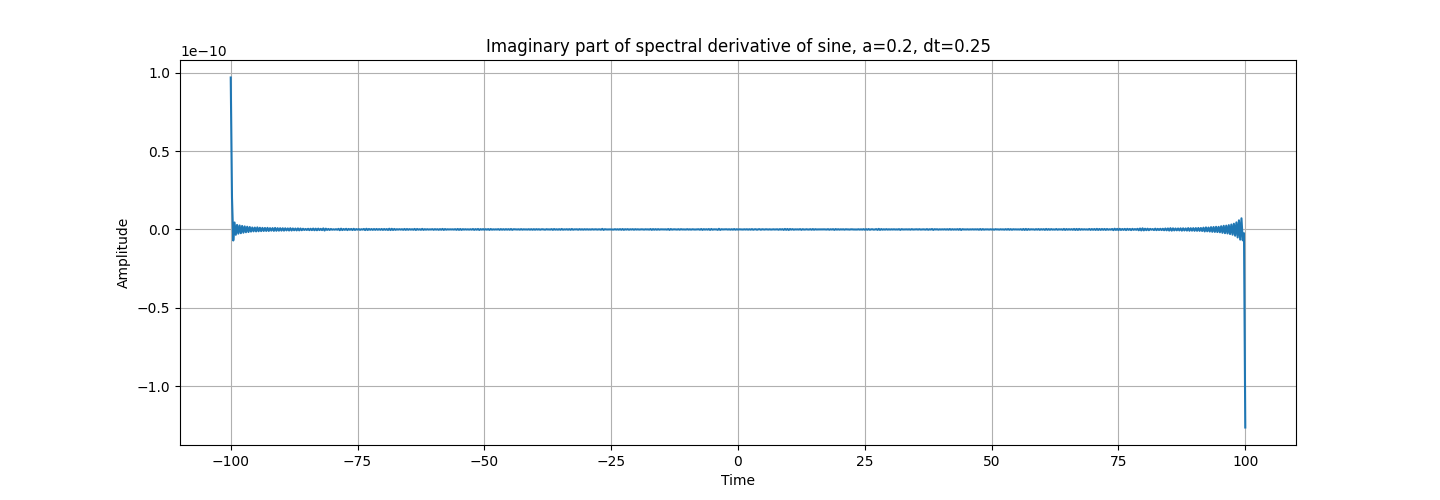
\includegraphics[scale=0.4]{1_im_specdiff_sine.png}
        \captionsetup{skip=0pt}
        \caption{Мнимая часть спектральной производной зашумленного сигнала.}
        \label{fig:1imspd}
    \end{figure}
    Наличие мнимой части указывает на фазовый сдвиг сигнала. Попробуем определить этот сдвиг по формуле $$\phi=\arctan{\left(\frac{b}{a}\right)},$$
    где $a,\,b$ -- вещественная и мнимая компоненты некоторого $\mathcal{F}_n\left\{\frac{d}{dt}f\right\}=a+ib$. Мы можем взять любую $n$, так как
    угол комплексного числа не меняется. Рассмотрим при $n=0$. $$\mathcal{F}_0\left\{\dfrac{d}{dt}f\right\}=7.17\cdot 10^{-12}-1.42i\Rightarrow
    \phi=-\dfrac{1.42}{7.17\cdot 10^{-12}}\approx -1.57 \approx -\dfrac{\pi}{2}.$$ Выходит, что спектральная производная сдвинула сигнал примерно
    на $90^{\circ}$. Позже мы проверим нашу теорию.
    На графике мнимой компоненты спектральной производной мы также наблюдаем пики при $t=-100,\,t=100$, что % todo
\end{document}